\documentclass[jair,twoside,11pt,theapa]{article}
\usepackage{jair, theapa, rawfonts}
\usepackage{graphicx}  % include figures
\usepackage{amsmath}  % for centering equations

\jairheading{?}{YYYY}{1-??}{M/YY}{M/YY}
\ShortHeadings{Standard Machine Learning Language}
{Ikegwu, Hao, \& Brunner}
\firstpageno{1}

\begin{document}

\title{Standard Machine Learning Language: A Language Agnostic Framework for Streamlining the Development of Machine Learning Pipelines}

\author{\name Kelechi Ikegwu \email ikegwu2@illinois.edu \\
       \addr 226 Astronomy Building, MC-124 \\1002 W. Green St.\\ Urbana, IL  61801
       \AND
       \name Micheal Hao  \email mxhao2@illinois.edu \\
       \addr ECE Building \\306 N Wright St. \\ Urbana, IL 61801
       \AND
       \name Robert Brunner \email bigdog@illinois.edu\\
       \addr 226 Astronomy Building, MC-221 \\1002 W. Green St.\\ Urbana, IL  61801}

% For research notes, remove the comment character in the line below.
% \researchnote

\maketitle


\begin{abstract}
Standard Machine Learning Language (SML) is a language agnostic framework that integrates a query-like language to simplify the development of machine learning pipelines. Emphasis was placed on ease of use and abstracting the complexities of machine learning from the end user encouraging it's use in professional and academic settings for a variety of disciplines. SML's architecture is discussed, followed by multiple interfaces that one could use to interact with SML. We then apply SML to a few problems and compare the complexities of SML queries and traditional approaches used to solve problems. Lastly we perform a case study on SML.
\end{abstract}

\section{Introduction}
\label{Introduction}

Machine Learning has simplified the process of solving a vast amount problems in a variety of fields by learning from data. In most cases machine learning has become more attractive than manually creating programs to solve these same issues. However there's a multitude of nuisances involved when developing machine learning pipelines \cite{pedros:fewUsefulThings}. If these nuisances are not taken into consideration one may not receive satisfactory results. A novice with domain knowledge utilizing machine learning to solve a particular problem may not want or have the time to deal with these complexities. To combat these issues we introduce Standard Machine Learning Language (SML).

The overall objective of the SML is to provide a level of abstraction which simplifies the development process of machine learning pipelines. Consequently this enables students, researchers, and industry professionals without a background in machine learning to solve problems in different domains with machine learning. We developed SML a query like language which serves as an abstraction from writing a lot of code (see Figure \ref{fig:sml-ex-1} for an example). In the subsequent sections related works are discussed followed by defining the grammar used to create queries for SML. The architecture of SML is described, lastly SML is applied to use-cases to demonstrate how it reduces the complexity of solving problems that utilize machine learning.

\begin{figure}
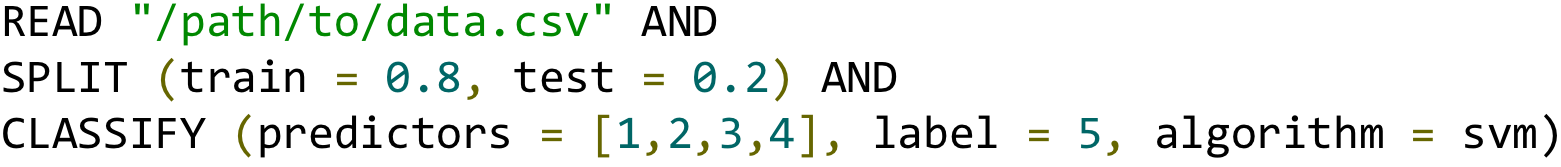
\includegraphics[width=0.6\textwidth]{figs/sml-ex-1.png}
\centering
\caption{Example of a SML Query performing classification.}
\label{fig:sml-ex-1}
\end{figure}

\section{Related Works}
\label{RelatedWorks}

They're related works that attempt to provide a level of abstraction as well for writing machine learning code. TPOT \cite{TPOT} is a tool implemented in python that creates and optimizes machine learning pipelines using genetic programming. Given cleaned data, TPOT performs feature selection, preprocessing , and construction. Given the task (classification, regression, or clustering) it uses the best features to determine the most optimal model to use. Lastly, it performs optimization on parameters for the selected model. What differentiates SML from TPOT is that in addition to feature, model, and parameter selection/optimization a framework is in place to apply these models to different datasets and construct visualizations for different metrics with each algorithm.

LBJava \cite{RizzoloRo10} is another tool  based on a programming paradigm called Learning Based Programming \cite{Roth05} which is an extension of conventional programming that creates functions using data driven approaches. LBJava follows the principles of learning based programming by abstracting the details of common machine learning processes. What separates SML from LBJava is that we offer a higher level of abstraction by providing a query like language which allows people who aren't experienced programmers to use SML.

\section{Grammar}
\label{grammar}

The SML language is a domain specific language with grammar implemented in Bakus-Naur form (BNF). Each expression has a rule and can be expanded into other terms. Figure \ref{fig:sml-ex-1} is an example of how one would perform classification on a dataset using SML. The query in Figure \ref{fig:sml-ex-1} reads from a dataset, performs a 80/20 split of training and testing data respectively, and performs classification on the 5th column of the hypothetical dataset using columns 1,2,3, and 4 as predictors. In the subsequent subsections SML's grammar in BNF form is defined in addition to the keywords.

\subsection{Grammar Structure}
This subsection is dedicated to defining the grammar of SML in terms of BNF. A \(Query\) can be defined by a delimited list of actions where the delimiter is an \(AND\) statement; with BNF syntax this is defined as:

\begin{equation} \label{BNF:Query}
<Query> ::= <Action> | <Action> AND <Query>
\end{equation}

An \(Action\) in (\ref{BNF:Query}) follows one of the following structures defined in (\ref{BNF:Action}) where a \(Keyword\) is required followed by an \(Argument\) and/or \(OptionList\).
\begin{equation} \label{BNF:Action}
\begin{split}
<Action> ::= <Keyword> “<Argument>” \\
| <Keyword> “<Argument>” “(”<Option List>“)” \\
| <Keyword> “(”<Option List>“)”
\end{split}
\end{equation}

A \(Keyword\) is a predefined term associating an \(Action\) with a particular string. An \(Argument\) generally is a single string surrounded by quotes that specifies a path to a file. Lastly, an \(Argument\) can have a multitude of options (\ref{BNF:Option}) where an \(Option\) consist of an \(OptionName\) with either an \(OptionValue\) or \(OptionValueList\). An \(OptionName\), and \(OptionValue\) consist of a single string, an \(OptionList\) (\ref{BNF:OptionList}) consist of a comma delimited list of options and an \(OptionValueList\) (\ref{BNF:OptionValueList}) consist of a comma delimited list of \(OptionValues\).

\begin{equation} \label{BNF:Option}
\begin{split}
<Option> ::= <Option Name> “=” <Option Value> \\
		| <Option Name> “=” “[”<Option Value List>“]”
\end{split}
\end{equation}

\begin{equation} \label{BNF:OptionList}
\begin{split}
	<Option List> ::= <Option> | <Option> “,” <Option List>
\end{split}
\end{equation}

\begin{equation} \label{BNF:OptionValueList}
\begin{split}
<Option Value List> ::= <Option Value> \\
| <Option Value> “,” <Option Value List>
\end{split}
\end{equation}

To put the grammar into perspective the example \(Query\) in Figure \ref{fig:sml-ex-1} has been transcribed into BNF format and can be found in Figure \ref{fig:SML:BNFComp}. The next subsection describes the functionality for all  \(Keyword\)s of SML.

\begin{figure}
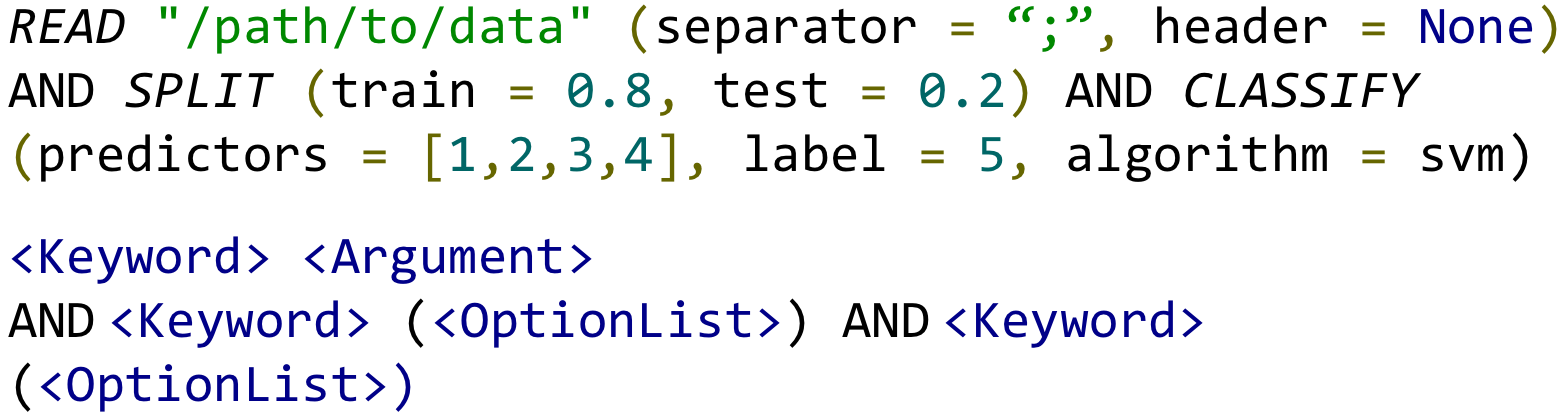
\includegraphics[width=0.6\textwidth]{figs/bnf_ex.png}
\centering
\caption{Transcribing Figure \ref{fig:sml-ex-1} into BNF form. Where the top \(Query\) was defined in Figure \ref{fig:sml-ex-1} and the bottom \(Query\) is in BNF format.}
\label{fig:SML:BNFComp}
\end{figure}


\subsection{Keywords}
Currently they're 8 \(Keyword\)s in SML \footnote{Detailed documentation providing examples and describing all of the keywords of SML are publicly available on github: https://github.com/lcdm-uiuc/sml/tree/master/dataflows \label{SML:Dataflow}}. These \(Keyword\)s can be chained together to perform a variety of actions. In the subsequent subsections we describe the functionality of each \(Keyword\).

\subsubsection{Reading Datasets}
When reading data from SML one must use the \(READ\) \(Keyword\) followed by an \(Argument\) containing a path to the dataset. \(READ\) also accepts an \(OptionList\). The first \(Query\) in Figure \ref{fig:SML:READ} consist of only a \(Keyword\) and \(Argument\). This \(Query\) reads in data from "/path/to/dataset". The second \(Query\) includes an \(OptionList\) in addition to reading data from the specified path; the \(OptionList\) specifies that the dataset is delimited with semicolons and does not include a header row. 

\begin{figure}

\includegraphics[width=0.6\textwidth]{figs/READ.png}
\centering
\caption{Example using the \(READ\) \(Keyword\) in SML.}
\label{fig:SML:READ}
\end{figure}

\subsubsection{Cleaning Data}
When NaNs, NAs and/or other troublesome values are present in dataset we clean these values in SML by using the \(REPLACE\) \(Keyword\).  Figure \ref{fig:SML:REPLACE}  shows an example of the \(REPLACE\) \(Keyword\) being used. In this \(Query\) we use the \(REPLACE\) \(Keyword\) in conjugation with the \(READ\) \(Keyword\). SML reads from a comma delimited dataset with no header from the path "/path/to/dataset". Then we replace any instance of "NaN" with the mode of that column in the dataset.

\begin{figure}

\includegraphics[width=0.6\textwidth]{figs/REPLACE.png}
\centering
\caption{Example of an SML \(Query\) being used.}
\label{fig:SML:REPLACE}
\end{figure}

\subsubsection{Partitioning Datasets}
It's often useful to split a dataset into training and testing datasets for most tasks involving machine learning. This can be achieved in SML by using the \(SPLIT\) \(Keyword\). Figure \ref{fig:SML:SPLIT} shows an example of a SML \(Query\) performing a 80/20 split for training and testing data respectively by utilizing the \(SPLIT\) \(Keyword\) after reading in data.

\begin{figure}
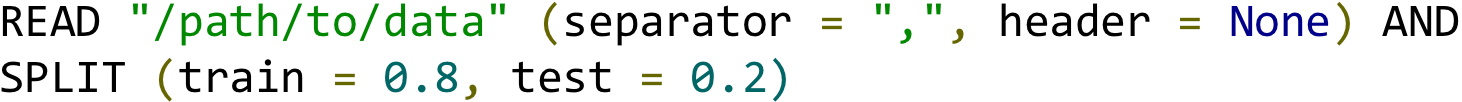
\includegraphics[width=0.6\textwidth]{figs/SPLIT.png}
\centering
\caption{Example using the \(SPLIT\) \(Keyword\) in SML.}
\label{fig:SML:SPLIT}
\end{figure}

\subsubsection{Using Classification Algorithms}
To use a classification algorithm in SML one would use the \(CLASSIFY\) \(Keyword\). SML has the following classification algorithms implemented: Support Vector Machines, Naive Bayes, Random Forest, Logistic Regression, and K-Nearest Neighbors. Figure \ref{fig:SML:CLASSIFY} demonstrates how to use the \(CLASSIFY\) \(Keyword\) in a \(Query\). 

\begin{figure}
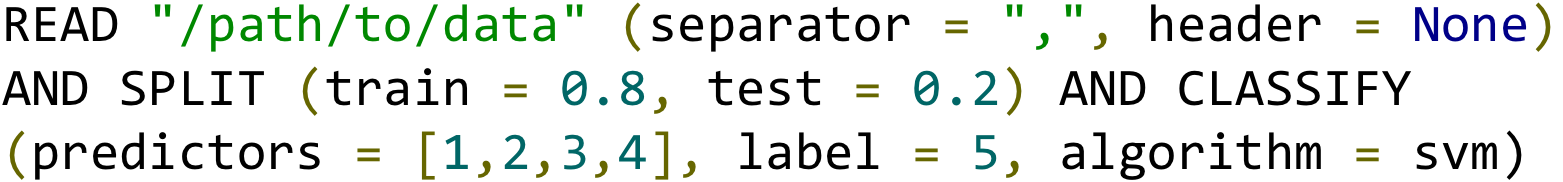
\includegraphics[width=0.6\textwidth]{figs/CLASSIFY.png}
\centering
\caption{Example using the \(CLASSIFY\) \(Keyword\) in SML. Here we read in data and create training and testing datasets using the \(READ\) and \(SPLIT\) \(Keyword\)s respectively. We then use \(CLASSIFY\) \(Keyword\) with the first 4 columns as features and the 5th column to perform classification using a support vector machine.}
\label{fig:SML:CLASSIFY}
\end{figure}

\subsubsection{Using Clustering Algorithms}
Clustering algorithms can be invoked by using the \(CLUSTER\) \(Keyword\). SML currently has K-Means clustering implemented. Figure \ref{fig:SML:CLUSTER} demonstrates how to use the \(CLUSTER\) \(Keyword\) in a \(Query\).

\begin{figure}
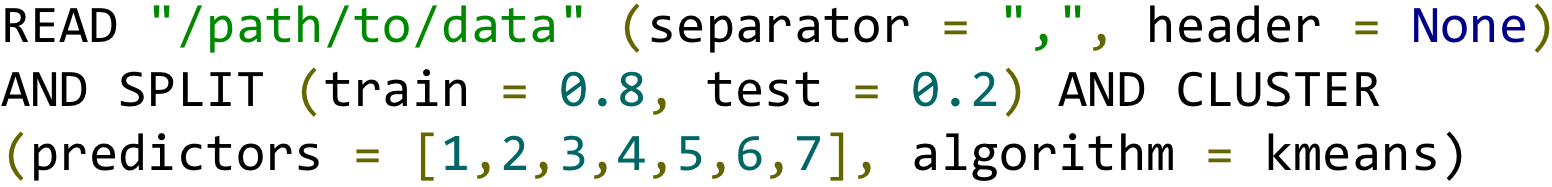
\includegraphics[width=0.6\textwidth]{figs/CLUSTER.png}
\centering
\caption{Example using the \(CLUSTER\) \(Keyword\) in SML. Here we read in data and create training and testing datasets using the \(READ\) and \(SPLIT\) \(Keyword\)s respectively. We then use \(CLUSTER\) \(Keyword\) with the first 7 columns as features and perform unsupervised clustering with the K-Means algorithm.}
\label{fig:SML:CLUSTER}
\end{figure}

\subsubsection{Using Regression Algorithms}
Regression algorithms use the \(REGRESS\) \(Keyword\). SML currently has the following regression algorithms implemented:Simple Linear Regression, Ridge Regression, Lasso Regression, and Elastic Net Regression. Figure \ref{fig:SML:REGRESS} demonstrates how to use the \(REGRESS\) \(Keyword\) in a \(Query\).

\begin{figure}
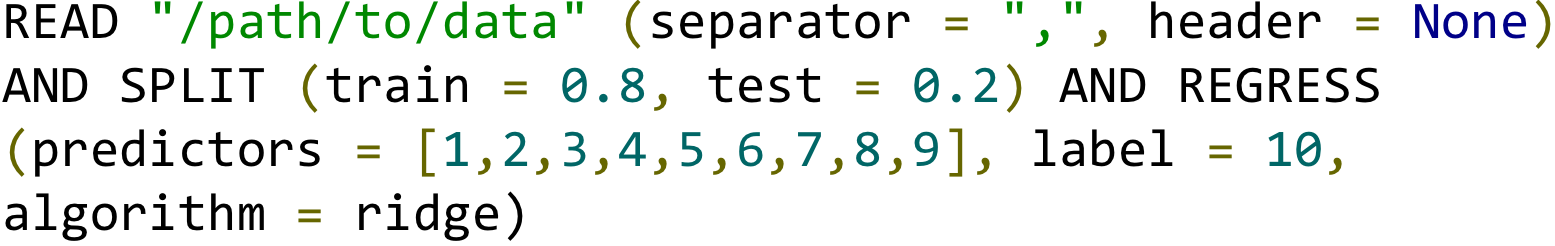
\includegraphics[width=0.6\textwidth]{figs/REGRESS.png}
\centering
\caption{Example using the \(REGRESS\) \(Keyword\) in SML. Here we read in data and create training and testing datasets using the \(READ\) and \(SPLIT\) \(Keyword\)s respectively. We then use \(REGRESS\) \(Keyword\) with the first 9 columns as features and the 10th column to perform regression on using ridge regression.}
\label{fig:SML:REGRESS}
\end{figure}

\subsubsection{Saving/Loading Models}
It's possible to save models and reuse them later. To save a model in SML one would use the \(SAVE\) \(Keyword\) in a \(Query\). To load an existing model from SML one would use the \(LOAD\) \(Keyword\) in a \(Query\). Figure \ref{fig:SML:SAVE_LOAD} shows how the syntax required save and load a model using SML. With any of the existing queries using \(REGRESS\), \(CLUSTER\), or \(CLASSIFY\) \(Keyword\)s attaching \(SAVE\) to the \(Query\) will save the model. 

\begin{figure}
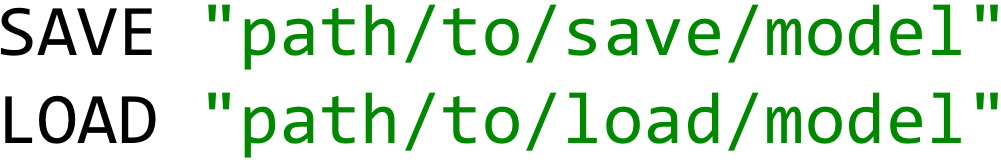
\includegraphics[width=0.3\textwidth]{figs/SAVE_LOAD.png}
\centering
\caption{Example using the \(LOAD\) and \(SAVE\) \(Keyword\)s in SML.}
\label{fig:SML:SAVE_LOAD}
\end{figure}

\subsubsection{Visualizing Datasets and Metrics of Algorithms}
When using SML it's possible to visualize datasets or metrics of algorithms (such as learning curves, or ROC curves). To do this the \(PLOT\) \(Keyword\) must be specified in a \(Query\). Figure \ref{fig:SML:PLOT} shows can example of how to use the \(PLOT\) \(Keyword\) in a \(Query\). We apply the same operations to perform clustering in Figure \ref{fig:SML:CLUSTER} however we utilize the \(PLOT\) \(Keyword\).

\begin{figure}
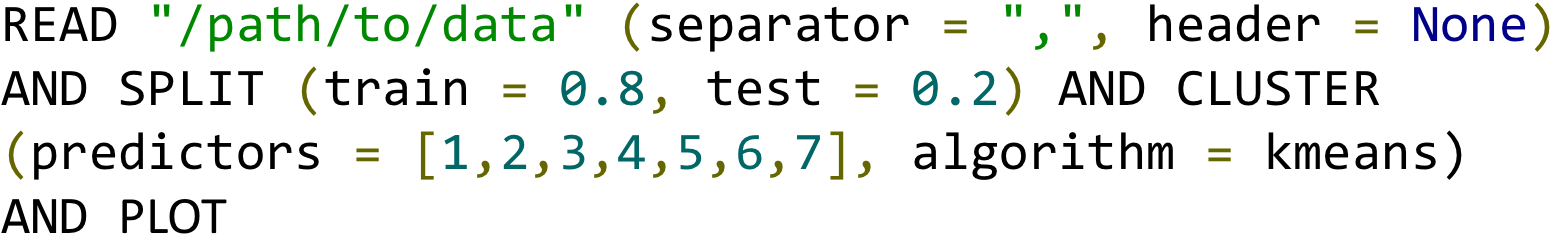
\includegraphics[width=0.6\textwidth]{figs/PLOT.png}
\centering
\caption{Example using the \(PLOT\) \(Keyword\) in SML.}
\label{fig:SML:PLOT}
\end{figure}

\section{SML's Architecture}
\label{sml-architecture}

With SML's grammar defined enough information has been presented to dive into SML's architecture. When SML is given a \(Query\) in the form of a string, it is passed to the parser. The high level implementation of the grammar is then used to parse through the string to determine the actions to perform. The actions are stored in a dictionary and given to one of the following phases of SML: Model Phase, Apply Phase, or Metrics Phase. Figure \ref{fig:SML:Architecture} shows a block diagram of this process.

\begin{figure}
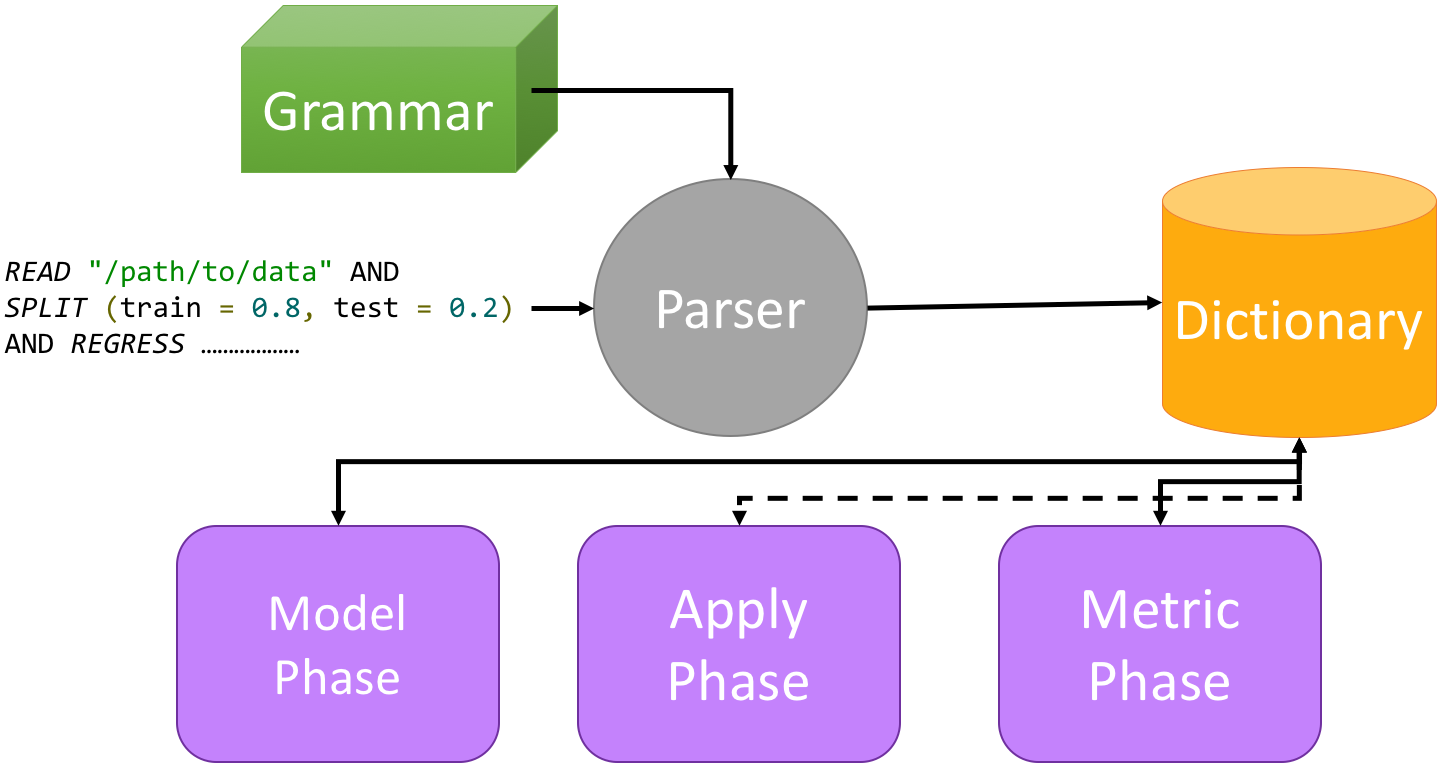
\includegraphics[width=0.6\textwidth]{figs/architecture.png}
\centering
\caption{Block Diagram of SML's Architecture}
\label{fig:SML:Architecture}
\end{figure}

The model phase is generally for constructing a model. The \(Keyword\)s that generally invoke the model phase are: \(READ\), \(REPLACE\), \(CLASSIFY\), \(REGRESS\), \(CLUSTER\), and \(SAVE\). The apply phase is generally for applying a preexisting model  to new data. The \(Keyword\)s that generally invoke the apply phase are: \(LOAD\), and \(APPLY\). It's often useful to visualize the data that one works with and beneficial to see performance metrics of a machine learning model. By default if you specify the \(PLOT\) \(Keyword\) in a \(Query\), SML will execute the metrics phase.

The last significant component of SML's architecture is the connector. The connector connects drivers from different libraries and languages to achieve an action a user want during a particular phase (see Figure \ref{fig:SML:Connector}). If one considers applying linear regression on a dataset, during the model phase SML calls the connector to retrieve the linear regression library in this case SML uses sci-kit learn's implementation however, if we wanted to use an an algorithm not available in sci-kit learn such as a Hidden Markov Model (HMM) SML will use the connector to call another library that supports HMM.

\begin{figure}
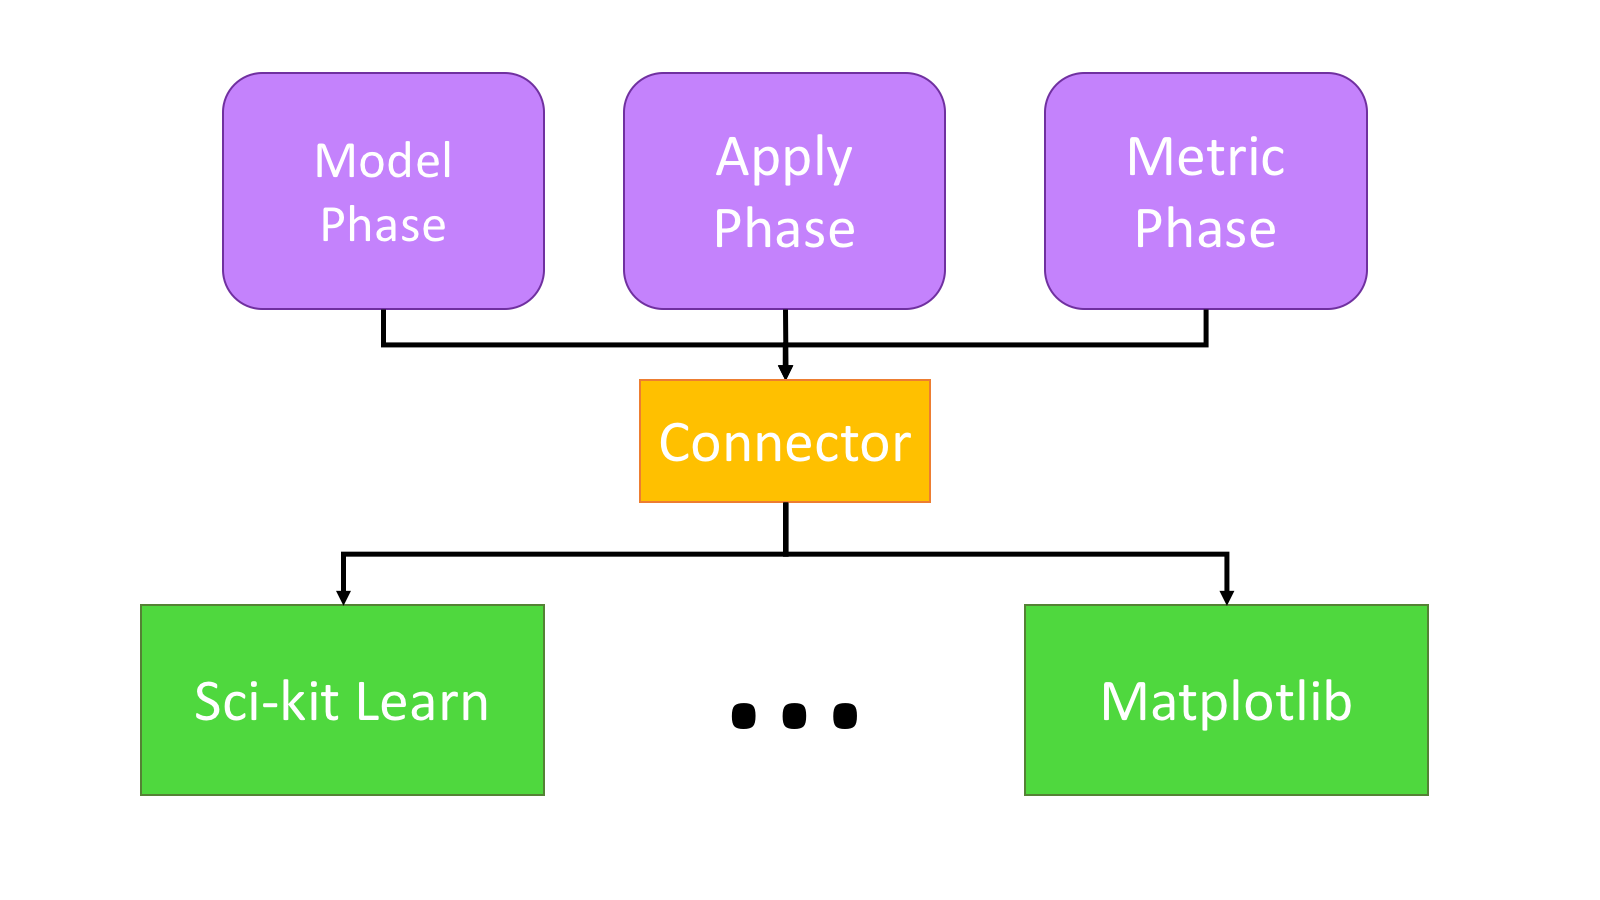
\includegraphics[width=0.6\textwidth]{figs/connector.png}
\centering
\caption{Block Diagram of SML's Connector}
\label{fig:SML:Connector}
\end{figure}

\section{Interface}
\label{interface}

They're multiple interfaces available for working with SML. We've developed a web tool that's publicly available which allows users to write queries and get results back from SML through a web interface (see Figure \ref{fig:SML:website}). There's also a REPL environment available that allows the user to interactively write queries and displays results from the appropriate phases of SML. Lastly, users have the option to import SML into an existing pipeline to simplify the development process of apply machine learning to problems.

\begin{figure}
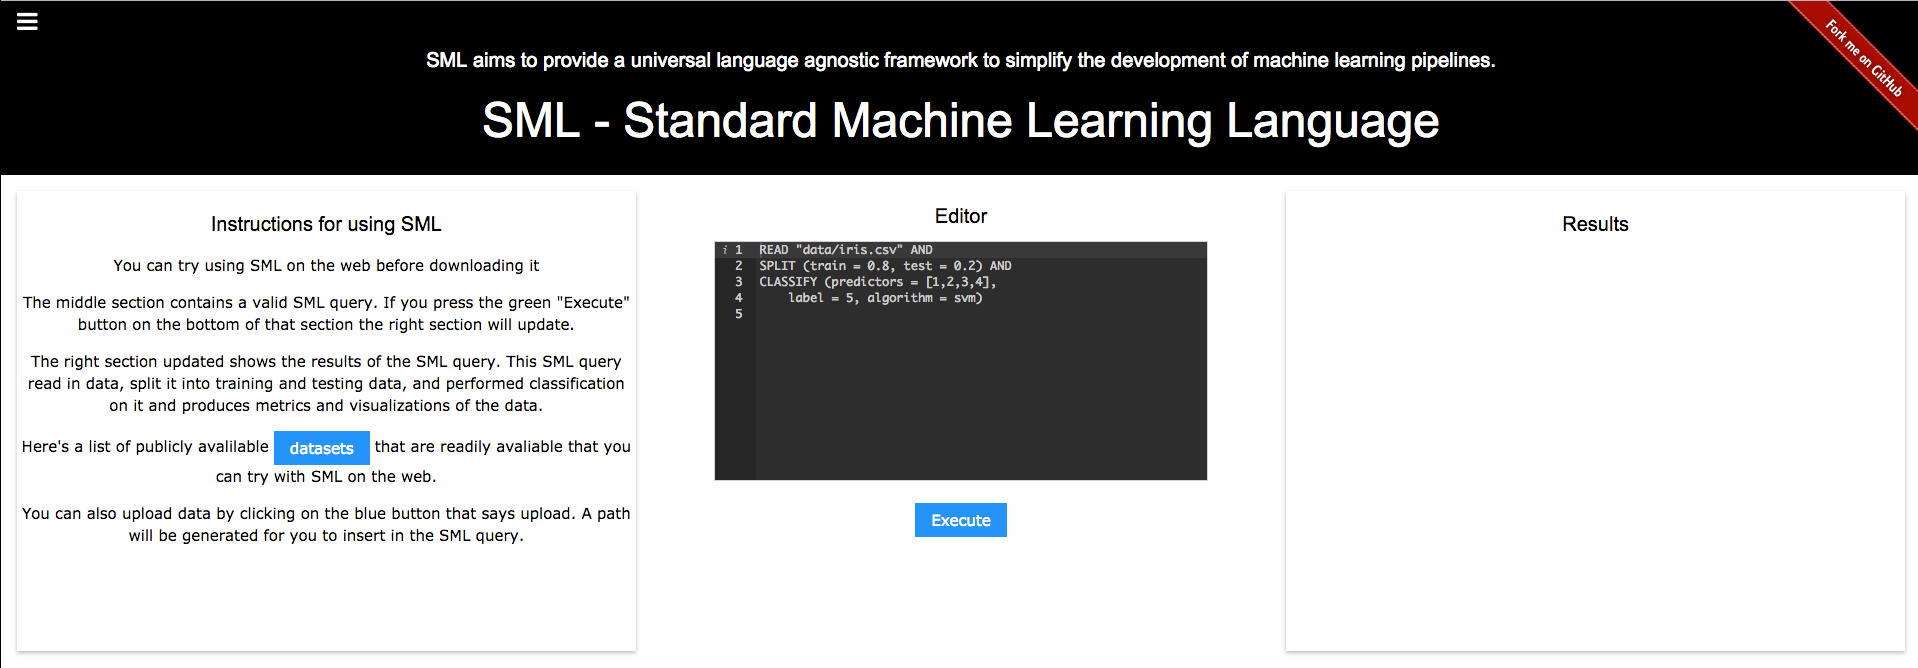
\includegraphics[width=0.6\textwidth]{figs/sml-web-site.png}
\centering
\caption{Interface of SML website. The user to interact with SML through a web interface (see Figure \ref{fig:SML:website}). Currently users can read instructions on the right to see examples of how to use SML. In the middle pane users can type SML Queries and then hit the execute button. The results of the \(Query\) are explained on the right pane.}
\label{fig:SML:website}
\end{figure}

\section{Use Cases}
\label{use-cases}

We tested the SML framework against ten popular machine learning problems with publicly available data sets. We applied SML to the following datasets: Iris Dataset \footnote{https://archive.ics.uci.edu/ml/datasets/Iris}, Auto-MPG Dataset \footnote{https://archive.ics.uci.edu/ml/datasets/Auto+MPG}, Seeds Dataset \footnote{https://archive.ics.uci.edu/ml/datasets/seeds}, Computer Hardware Dataset \footnote{https://archive.ics.uci.edu/ml/datasets/Computer+Hardware}, Boston Housing Dataset \footnote{https://archive.ics.uci.edu/ml/datasets/Housing}, Wine Recognition Dataset \footnote{https://archive.ics.uci.edu/ml/datasets/Wine}, US Census Dataset \footnote{https://archive.ics.uci.edu/ml/datasets/US+Census+Data+(1990)}, Chronic Kidney Disease \footnote{https://archive.ics.uci.edu/ml/datasets/Chronic\_Kidney\_Disease}, Spam Detection \footnote{https://archive.ics.uci.edu/ml/datasets/Spambase} which were taken from UCI's Machine Learning Repository \cite{Lichman:2013}. We also applied SML to the Titanic Dataset \footnote{https://www.kaggle.com/c/titanic}. In this paper we discuss in detail the process of applying SML to the Iris Dataset and the Auto-MPG dataset. \footnote{Footnote \ref{SML:Dataflow} provides detailed explanations and examples that solve problems all 10 data sets.}

\subsubsection{Iris Dataset}
Figure \ref{fig:SML:IrisQuery} shows all of the code required to perform classification on the Iris dataset. In Figure \ref{fig:SML:IrisQuery} data is read in from a specified path of a file called "iris.csv" of a subdirectory called "data" in the parent directory, perform a 80/20 split, use the first 4 columns to predict the 5th column, use support vector machines as the algorithm to perform classification and finally plot distributions of our dataset  and metrics of our algorithm. Figure \ref{fig:Manual:IrisCode} illustrates what is required to perform the same operations using scikit learn. The \(Query\) in Figure \ref{fig:SML:IrisQuery} and Figure \ref{fig:Manual:IrisCode} use the same 3rd party libraries implicitly or explicitly. It's worth noting that the code in Figure \ref{fig:Manual:IrisCode} is publicly available and well documented \footnote{For a detailed documentation describing this code visit: https://github.com/lcdm-uiuc/sml/blob/master/dataflows/plot/iris\_svm-READ-SPLIT-CLASSIFY-PLOT.ipynb} and it is out of the scope of this paper. Instead the complexities required to produce such results with and without SML are outlined. The result for both snippets of code are the same and can be seen in Figure \ref{fig:IrisResults}.

\begin{figure}
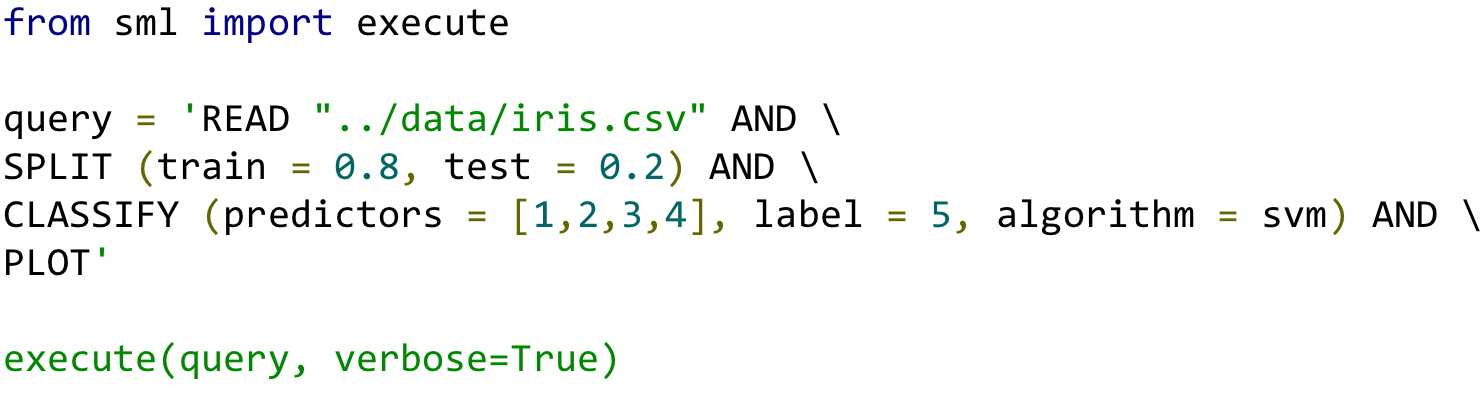
\includegraphics[width=0.6\textwidth]{figs/iris_sml.png}
\centering
\caption{SML \(Query\) that performs classification on the iris dataset using support vector machines.}
\label{fig:SML:IrisQuery}
\end{figure}

\begin{figure}
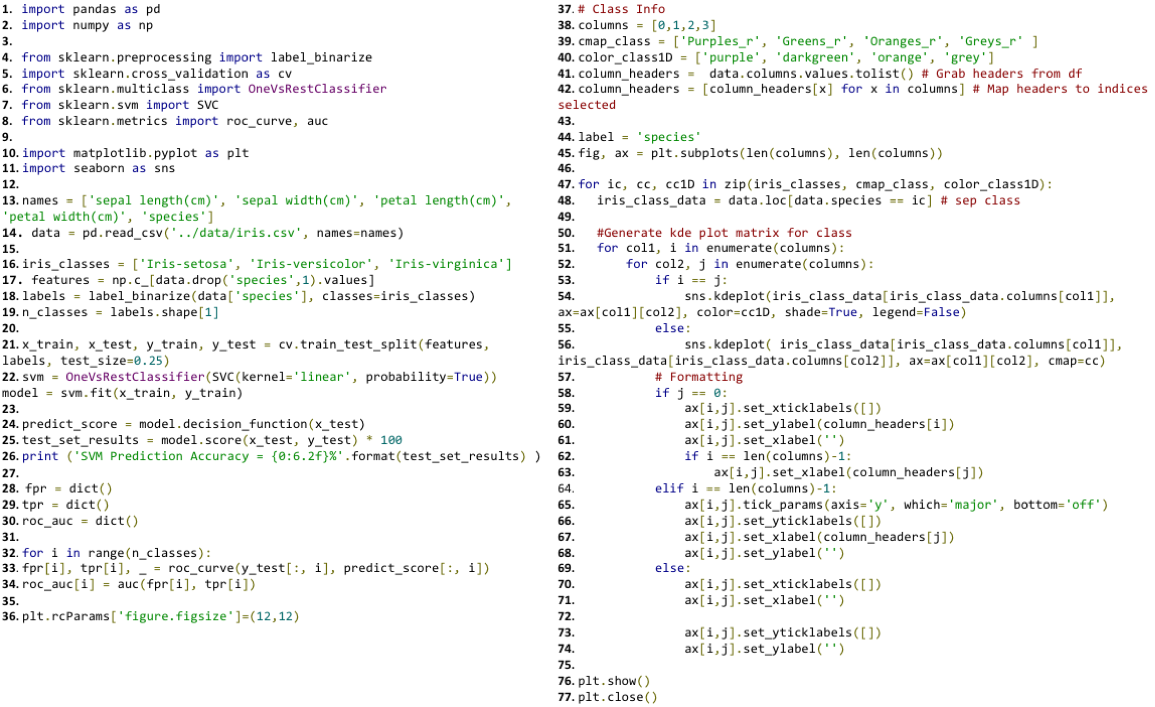
\includegraphics[width=0.6\textwidth]{figs/iris_manual.png}
\centering
\caption{This shows the code required to replicate the same actions of the SML \(Query\) in Figure \ref{fig:SML:IrisQuery}}
\label{fig:Manual:IrisCode}
\end{figure}

\begin{figure}
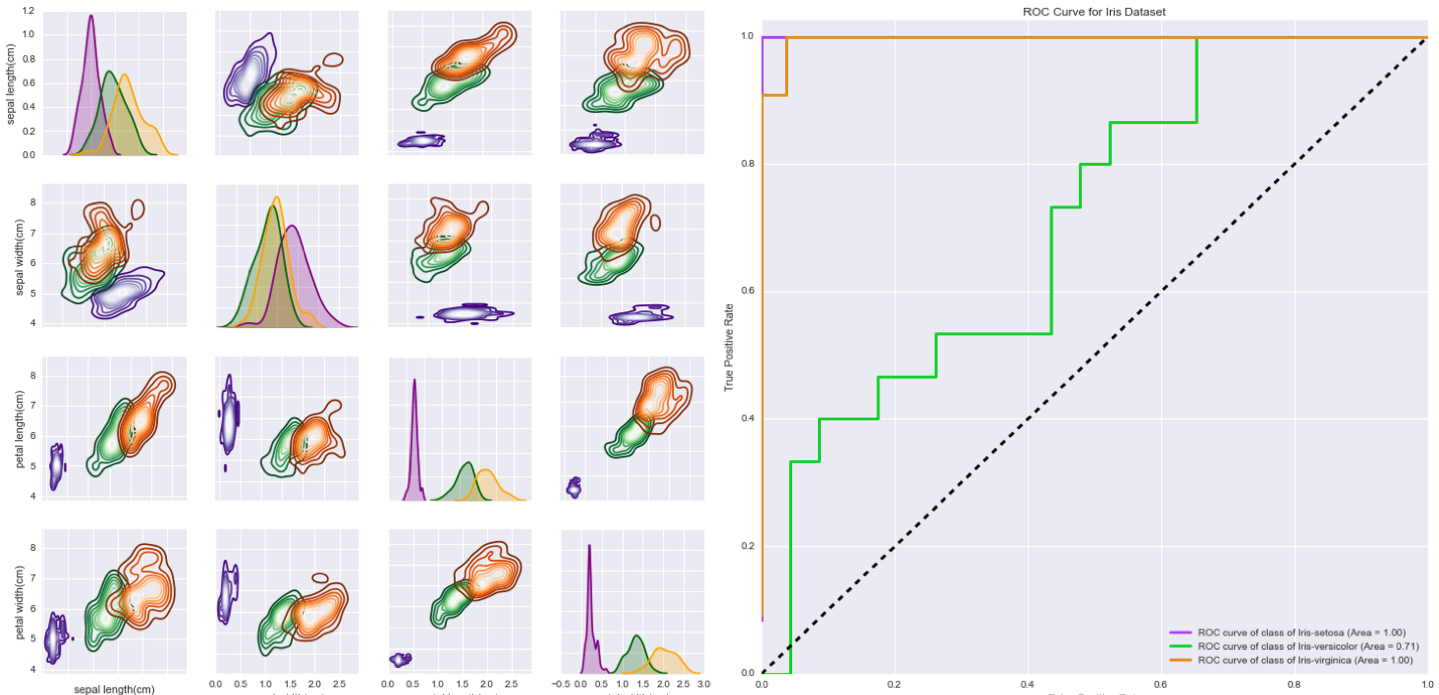
\includegraphics[width=0.6\textwidth]{figs/iris_results.png}
\centering
\caption{The SML \(Query\) in Figure \ref{fig:SML:IrisQuery} and the code in Figure \ref{fig:Manual:IrisCode} produce these results. The subgraph on the left is a lattice plot showing the density estimates of each feature used. The graph on the right shows the ROC curves for each class of the iris dataset.}
\label{fig:IrisResults}
\end{figure}


\subsubsection{Auto-Mpg Dataset}
Figure \ref{fig:SML:AutoMPGQuery} shows the SML \(Query\) required to perform regression on the Auto-MPG dataset. In Figure \ref{fig:SML:AutoMPGQuery} we read data from a specified path, the dataset is separated by fixed width spaces and we choose not to provide a header for the dataset.  Next we perform a 80/20 split, replace all occurrences of "?" with the mode of the column. We then perform linear regression using columns 2-8 to predict the 1st label. Lastly, we visualize distributions of our dataset and metrics of our algorithm. Figure \ref{fig:Manual:Auto-MPG} demonstrates what's required to perform the same operations using scikit learn \footnote{For a detailed documentation describing this code visit: https://github.com/lcdm-uiuc/sml/blob/master/dataflows/plot/autompg\_linear\_regression-READ-SPLIT-REGRESS-PLOT.ipynb}. The outcome for both process are the same and can be seen in Figure \ref{fig:AutoMPG:Results}.

\begin{figure}
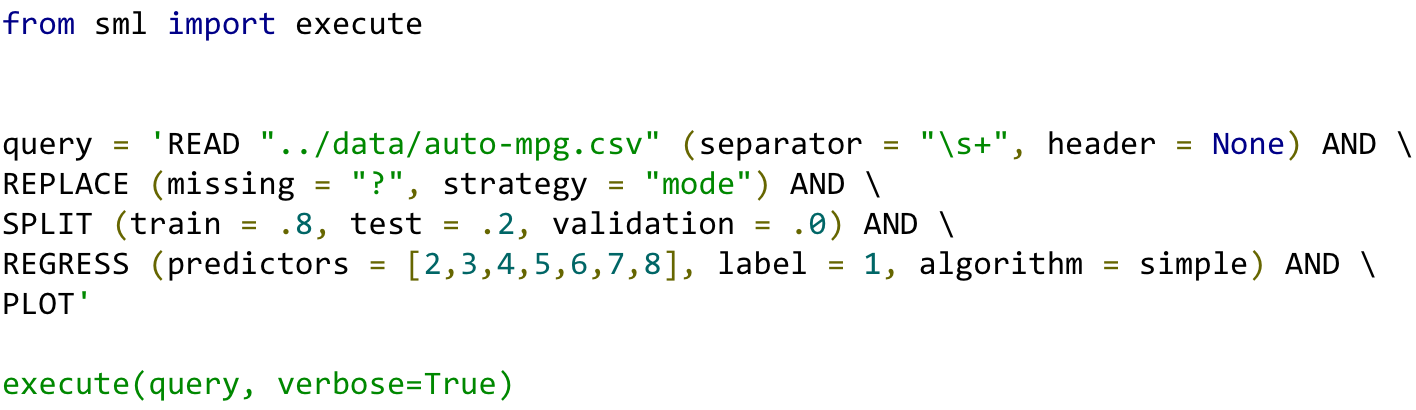
\includegraphics[width=0.6\textwidth]{figs/autompg_sml.png}
\centering
\caption{SML \(Query\) that performs classification on the Auto-MPG dataset using support vector machines.}
\label{fig:SML:AutoMPGQuery}
\end{figure}

\begin{figure}
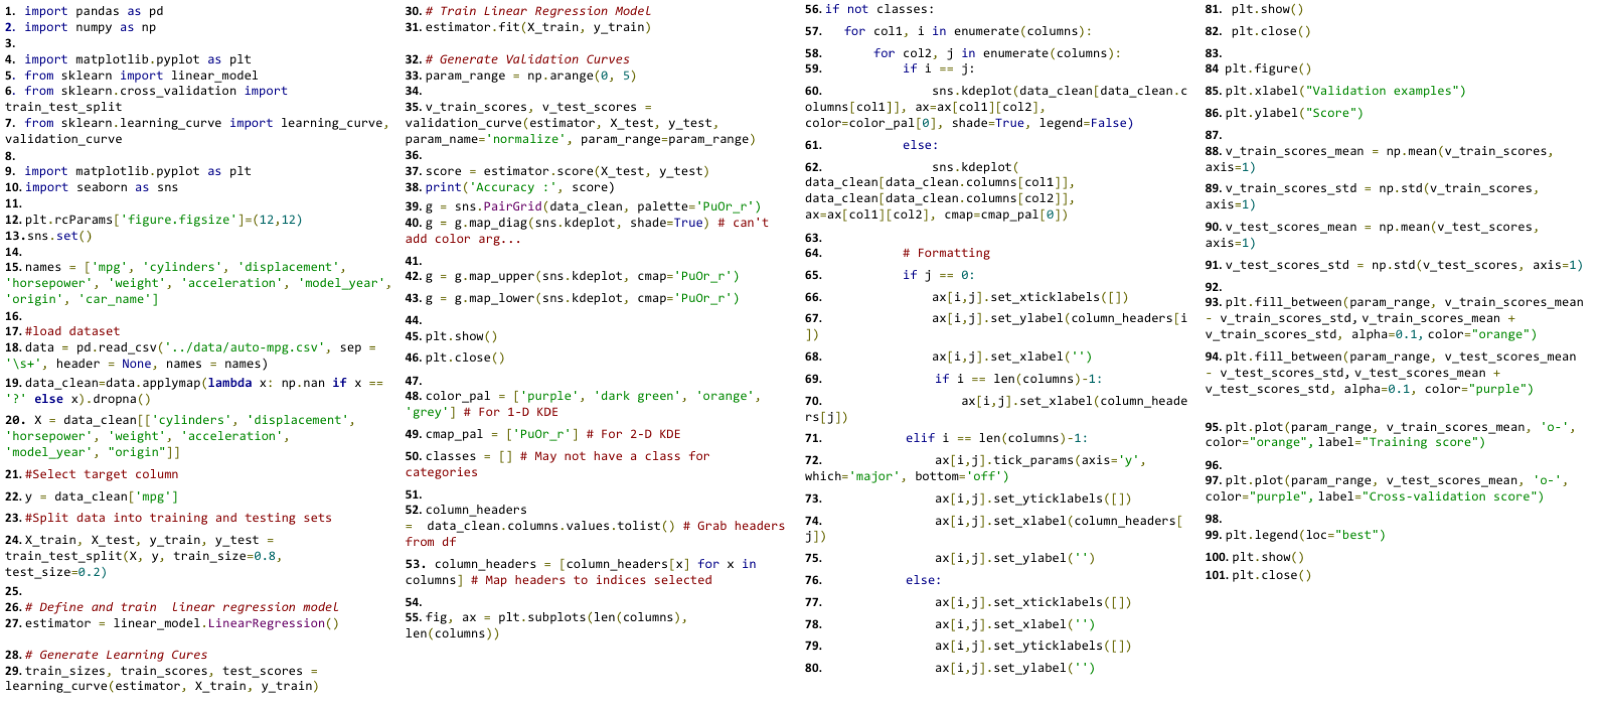
\includegraphics[width=0.6\textwidth]{figs/auto-mpg_manual.png}
\centering
\caption{This shows the code required to replicate the same actions of the SML \(Query\) in Figure \ref{fig:SML:AutoMPGQuery}}
\label{fig:Manual:Auto-MPG}
\end{figure}

\begin{figure}
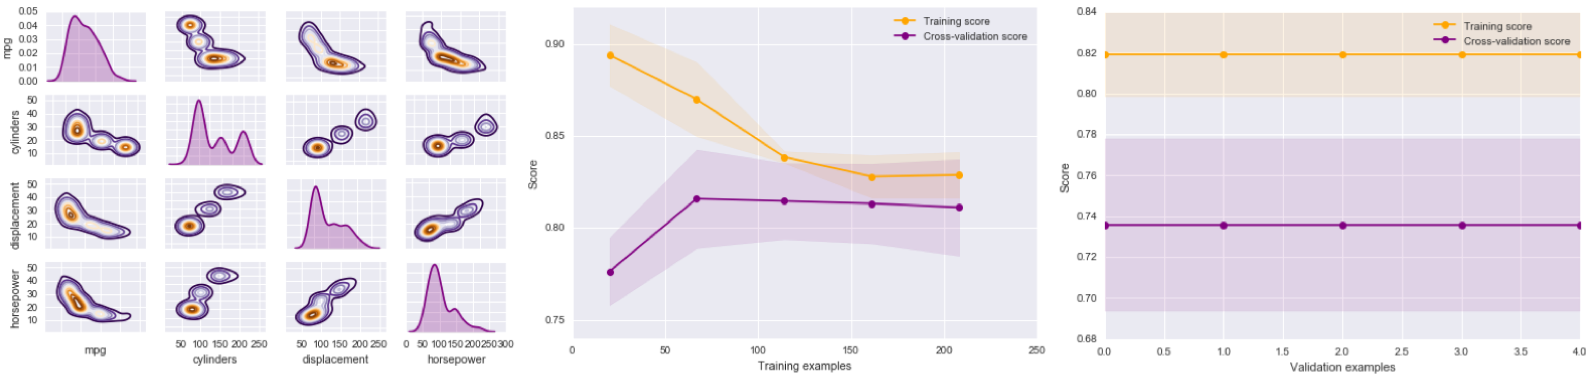
\includegraphics[width=0.6\textwidth]{figs/auto-mpg-results.png}
\centering
\caption{The SML \(Query\) in Figure \ref{fig:SML:AutoMPGQuery}  and the code in Figure \ref{fig:Manual:Auto-MPG} produce these results. The subgraph on the left is a lattice plot showing the density estimates of each feature used. The the centered shows the learning curve of the model and the graph on right shows the validation curve.}
\label{fig:AutoMPG:Results}
\end{figure}

\subsection{Discussion}
For the Iris and Auto-MPG use cases the same libraries were used to perform regression and classification. The amount of work require to perform a task and produce the following results in Figure \ref{fig:AutoMPG:Results} and Figure \ref{fig:IrisResults} significantly decreases when SML is utilized. To construct each of the SML queries less than 10 lines are required however, to implement the same procedures without SML using the same libraries 80+ lines are required. This demonstrates that it simplifies the development process of solving problems with machine learning and opens a realm of possibility to rapidly develop machine learning pipelines which would be an attractive aspect for researchers.

\section{Conclusion}
\label{conclusion}
To summarize we introduced an agnostic framework that integrates a query-like language to simplify the development of machine learning pipelines. We provided a high level overview of it's architecture and grammar. We then applied SML to machine learning problems and demonstrated how the complexity of the code one has to write significantly decreases when SML is used. The source code and detailed documentation for SML is open sourced and publicly available on github \footnote{https://github.com/lcdm-uiuc/sml \label{SML:Github}}. In the future we plan to extend the connector to support more machine learning libraries and additional languages. We plan to expand the web application to make SML easier to use.

If we want to researchers from other domain areas to utilize machine learning without understanding the complexities required for machine learning a tool like SML is needed. The concepts presented in this paper as a whole is sound. The details may change but the core principals will remain the same. Abstracting the complexities of machine learning from users are needed to increase the use of machine learning by researchers in different disciplines.


%\acks{acknowledgments go here}
%\appendix
%\section*{Appendix X...}
%Appendix goes here if needed.

\vskip 0.2in
\bibliography{main}
\bibliographystyle{theapa}

\end{document}






